% Drawing 144/05-3 -- folder 144, batch 05, archive page 90 (PDF page 91).
% Transcription: en marge, une sphère : le pôle $P_+$, sur l'équateur $R_0$, $Q_{a_0}$, $R_1$ ; les chemins $\alpha$ et $\tilde\sigma_{a_0}^0(\alpha) = \alpha'$ descendent vers $P$ et $P' = \tilde\sigma_{a_0}^0(P)$, reliés par $\tilde\alpha_\sigma$.
% Kind: sphere with paths alpha, alpha' and tilde alpha_sigma. Method 2 (schematic redraw from the facsimile). Status: ok.
% Notes: P_+ at the pole; R_0, Q_{a_0}, R_1 on the equator; the paths alpha and alpha' = tilde sigma^0_{a_0}(alpha) (dashed) descend from P_+ to P and P' = tilde sigma^0_{a_0}(P), joined by tilde alpha_sigma.
% Coordinates: 1 unit = 1 mm = 1/100 of the crop width (bbox in page fractions: [0.1, 0.66, 0.38, 0.8]).
% Redrawn by Claude (claude-opus-5-5), issue #73, 2026-11-07; not checked by a human; not compiled (no TeX in the session).
% Rights: reproduces part of the work -- behind RENDER_TRANSCRIPTS, never published by itself.
\documentclass[tikz,border=3pt]{standalone}
\usepackage{amsmath,amssymb}
\usetikzlibrary{patterns,arrows.meta}
\tikzset{pencil/.style={black!45}, struck/.style={black!35}, mark/.style={circle,draw,inner sep=1.3pt}, pt/.style={circle,fill,inner sep=0.9pt}, opt/.style={circle,draw,fill=white,inner sep=1.1pt}}
\begin{document}
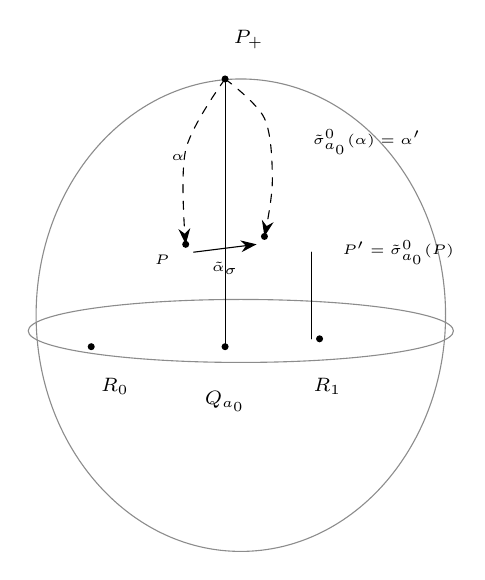
\begin{tikzpicture}[x=1mm,y=1mm,line cap=round,line join=round,font=\scriptsize]
\draw[pencil] (40,-45) ellipse[x radius=26, y radius=30];
\draw[pencil] (40,-47) ellipse[x radius=27, y radius=4];
\node[pt] at (38,-15) {};
\node[inner sep=1pt] at (41,-10) {\scriptsize $P_+$};
\draw[dashed,-{Stealth[length=2mm]}] plot[smooth, tension=0.55] coordinates {(38,-15) (33,-24) (33,-36)};
\draw plot[smooth, tension=0.55] coordinates {(38,-15) (38,-30) (38,-49)};
\draw[dashed,-{Stealth[length=2mm]}] plot[smooth, tension=0.55] coordinates {(38,-15) (43,-20) (44,-28) (43,-35)};
\draw (49,-37) -- (49,-48);
\node[pt] at (21,-49) {};
\node[pt] at (38,-49) {};
\node[pt] at (50,-48) {};
\node[pt] at (33,-36) {};
\node[pt] at (43,-35) {};
\draw[-{Stealth[length=2mm]}] (34,-37) -- (42,-36);
\node[inner sep=1pt] at (24,-54) {\scriptsize $R_0$};
\node[inner sep=1pt] at (38,-56) {\scriptsize $Q_{a_0}$};
\node[inner sep=1pt] at (51,-54) {\scriptsize $R_1$};
\node[inner sep=1pt] at (30,-38) {\tiny $P$};
\node[inner sep=1pt] at (32,-25) {\tiny $\alpha$};
\node[inner sep=1pt] at (38,-39) {\tiny $\tilde\alpha_\sigma$};
\node[inner sep=1pt] at (60,-37) {\tiny $P'=\tilde\sigma^0_{a_0}(P)$};
\node[inner sep=1pt] at (56,-23) {\tiny $\tilde\sigma^0_{a_0}(\alpha)=\alpha'$};
\end{tikzpicture}
\end{document}
